\chapter{相关工作以及技术}
本章介绍本文研究中涉及到的数据集和关键理论与技术。数据集主要包括Med-RAD和SLAKE两大Med-VQA数据集;关键理论与技术主要包括视觉问答技术、视觉问答系统、VQA中的编码技术原理,跨模态自注意力机制以及贝叶斯不确定性估计理论。

\section{视觉问答技术}
视觉问答\cite{antol2015vqa}(Visual Question Answering,VQA)是一种结合了计算机视觉和自然语言处理技术的交叉领域任务,其目标是让机器理解人类提出的关于图像内容的自然语言问题,并在语言层面上回答这些问题.如\ref{vqademo}所示,
与传统的图像识别任务相比,VQA需要综合考虑图像和问题两方面的信息,同时进行视觉推理和自然语言理解。
\begin{figure}[htbp]
	% 图片居中(列居中对齐)
	\centering	
	% 包含当前路径下的Fig文件夹的图片文件
	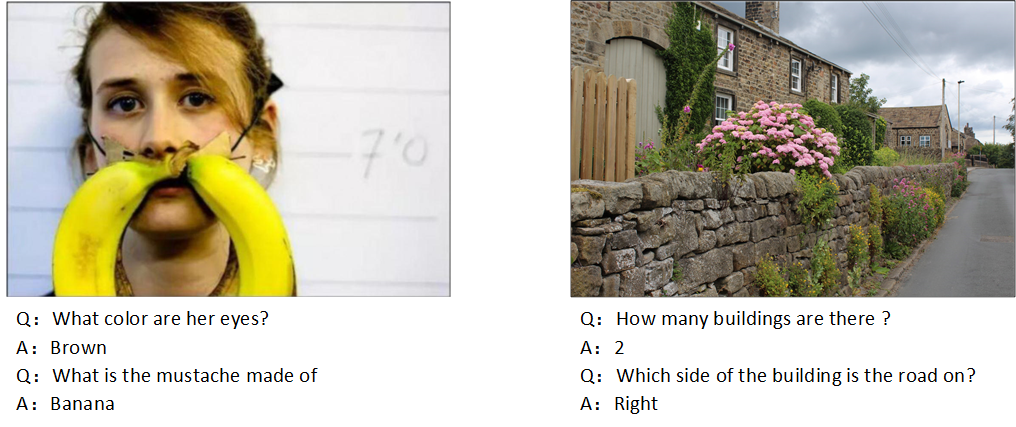
\includegraphics[width=1\textwidth]{Fig/myfig/chapter2/vqademo.png}  %scale = 0.3
	% 添加标签one_DFUAV以及图标题“XXX”,引用某图时使用\ref{xxx},其中xxx就是标签,图编号是自动生成的。
	\caption{\label{vqademo}视觉问答样例} 
\end{figure}

VQA技术的基本流程包括图像特征提取、问题特征提取、多模态融合和答案预测等步骤。其中,图像特征提取可以使用传统的卷积神经网络(CNN)模型或预训练的图像识别模型(如ResNet、Inception等)进行。
问题特征提取可以使用自然语言处理技术,例如词嵌入\cite{}(word embedding)和循环神经网络(RNN)等。多模态融合可以使用传统的融合方法,例如特征串联、特征相加等,也可以使用基于注意力机制的融合方法,
例如多头注意力、视觉注意力、文本注意力等。答案预测可以使用分类模型获得较为准确的结果,也可以使用生成模型获得更为灵活的回答。
% \begin{figure}[htbp]
% 	% 图片居中(列居中对齐)
% 	\centering	
% 	% 包含当前路径下的Fig文件夹的图片文件
% 	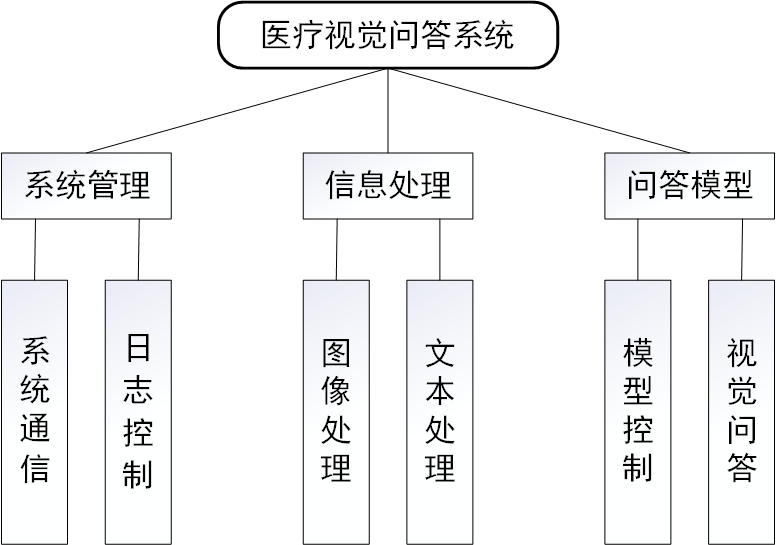
\includegraphics[width=0.8\textwidth]{Fig/myfig/chapter5/sys_need.png}  %scale = 0.3
% 	% 添加标签one_DFUAV以及图标题“XXX”,引用某图时使用\ref{xxx},其中xxx就是标签,图编号是自动生成的。
% 	\caption{\label{sys_need}需求分析} 
% \end{figure}

\section{医学视觉问答系统}
\subsection{医学视觉问答系统的组成}
如图\ref{sys_need}一个完整的视觉问答系统通常由七个主要组件组成:数据集、图像处理模块、自然语言处理模块、多模态融合模块、答案生成模块、前端应用以及后端服务器。
数据集是系统的基础,其质量决定了模型性能的好坏;为了更好的迭代模型以及提高系统的交互体验,一般还会给系统加入信息反馈机制,问答者可以对系统的回答做出评价
以及调整意见,模型在迭代时会根据反馈对回答机制和内容进行适当的调整,从而提高系统的整体性能。
\begin{figure}[htbp]
	% 图片居中(列居中对齐)
	\centering	
	% 包含当前路径下的Fig文件夹的图片文件
	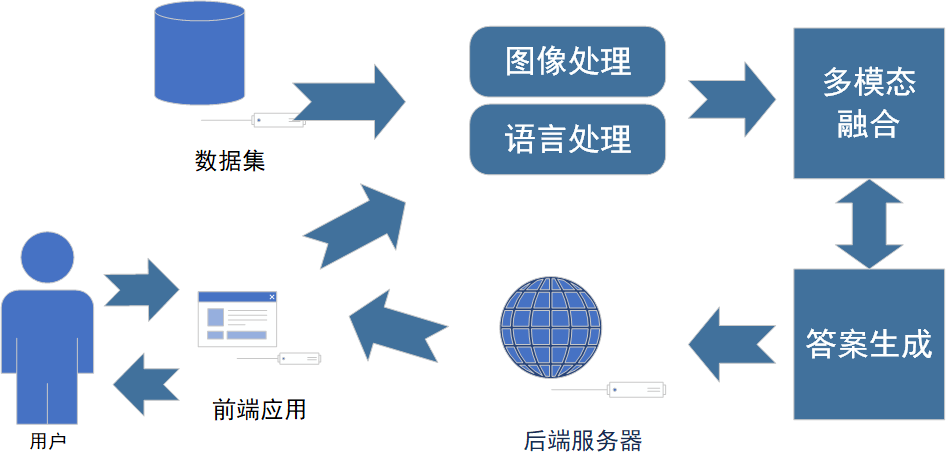
\includegraphics[width=0.8\textwidth]{Fig/myfig/chapter2/sys_vqa.png}  %scale = 0.3
	% 添加标签one_DFUAV以及图标题“XXX”,引用某图时使用\ref{xxx},其中xxx就是标签,图编号是自动生成的。
	\caption{\label{sys_need}视觉问答系统} 
\end{figure}

图像处理模块负责从输入的图像中提取有用的视觉特征;自然语言处理模块负责处理用户的自然语言输入,如问题或指令;多模态融合模块将图像特征向量和问题向量融合起来,以生成一个综合的向量表述;答案生成模块对融合后的向量进行预测,并生成一个符合语义和语法的答案。
前端应用为用户提供了一个界面来输入问题,并展示系统回答的答案。通常使用Web或移动应用程序来实现前端应用程序。后端服务器:后端服务器是视觉问答系统的核心部分,
它处理来自前端应用程序的请求,并将其传递给模型进行预测。后端服务接口通常使用API来实现。此外,一些系统还包括预处理模块,如图像分割和对象检测,这些组件的结合形成了一个完整的视觉问答服务系统,
可以用于各种应用,如智能客服、医疗诊断和自动驾驶。

\subsection{医学视觉问答系统的分类}
\begin{enumerate}[topsep = 0 pt, itemsep= 0 pt, parsep=0pt, partopsep=0pt, leftmargin=44pt, itemindent=0pt, labelsep=6pt, label=(\arabic*)]
    \item 根据应用领域的不同,由于医学图像种类、数量复杂繁多,可以按其应用分为多个不同的领域,如放射学、病理学、眼科等不同领域的系统。在放射学领域,医学视觉问答系统可以用于解读医学影像,如CT、MRI等,帮助医生诊断疾病。在病理学领域,医学视觉问答系统可以用于分析组织切片图像,帮助医生诊断肿瘤和其他疾病。在眼科领域,医学视觉问答系统可以用于识别和诊断眼部疾病,如白内障、青光眼等。不同领域的医学视觉问答系统所需的数据、特征提取方法、模型架构等都可能存在差异,因此需要专门针对不同领域进行研究和开发。
    \item 根据问答类型的不同,可以将医学视觉问答系统分为封闭式问答和开放式问答系统,封闭式问答是指问题的答案是事先给定的,系统只需要从给定的答案集合中选择正确的答案进行回答。这种问答方式的优点是简单高效,但是答案集合通常需要经过手动标注,且无法回答没有出现在答案集合中的问题。开放式问答则是指问题的答案不是事先给定的,系统需要从自然语言文本中寻找答案。这种问答方式的优点是可以回答更广泛的问题,但是也更加复杂和困难。开放式问答通常需要使用自然语言处理技术来理解问题和文本,以及对答案进行生成或者抽取。
    \item 根据系统实现的不同,可以划分为基于传统机器学习方法的系统和基于深度学习方法的系统。传统机器学习方法的系统通常包括以下步骤:首先,对图像和问题进行特征提取;然后,将两者的特征向量融合在一起;最后,使用机器学习模型(如支持向量机、随机森林等)进行分类或回归预测。这种方法的优点是较为简单,容易理解和解释,但其效果受限于手动设计的特征和模型。基于深度学习方法的系统则利用深度神经网络自动地学习图像和问题的特征表示,并将二者进行融合。
    常用的深度学习模型包括卷积神经网络(Convolutional Neural Networks,CNN)、循环神经网络(Recurrent Neural Networks,RNN)和注意力机制(Attention Mechanism)等。深度学习方法可以更好地利用数据的内在规律,提高模型的预测性能,但需要更多的计算资源和数据量,并且模型的可解释性较差。
    \item 根据系统目的的不同,可以划分为辅助医生诊断的系统、辅助患者自我诊断诊断的系统和用于医学教育等不同目的的系统。辅助医生的系统主要是为了协助医生对医学图像进行分析和诊断。这类系统需要针对医生所需要的信息提供准确的答案,帮助医生做出正确的诊断和治疗决策。例如,一些放射学视觉问答系统可以帮助放射科医生快速准确地分析和诊断CT、MRI等医学图像。帮助病人的系统主要是为了帮助病人在家中自我进行初步的诊断和监测。这类系统需要具有简单易用、普及率高的特点,让病人能够方便地获取自己的健康信息。例如,一些眼科视觉问答系统可以帮助病人自行检查眼部问题并获取相应的诊断和治疗建议。
    用于医学教育的系统主要目的是帮助医学教育工作者、学生和其他研究人员更好地学习和理解医学知识。这类系统需要提供丰富、准确的医学知识和信息,并且要具有易用性和可扩展性,以满足不同的学习需求。例如,一些病理学视觉问答系统可以帮助医学学生更好地理解组织病理学的知识,同时也可以为病理医生提供更快速、准确的诊断和治疗决策支持。
\end{enumerate}

\section{Med-VQA数据集}
医学视觉问答是一个新兴领域,且由于标准成本较高,与通用领域相比,现拥有的公开数据集十分稀少。其中的主要代表是VQA-Med、VQA-RAD、PATH、SLAKE这四个数据集。VQA-Med-2018\cite{hasan2018overview}是领域内第一个公开可用的数据集,
也是Med-VQA领域标准竞赛数据集。由于仅仅用于竞赛的原因,目前VQA-Med的缺陷是QA对是通过半自动化的方式生成的:由基于规则的问题生成系统(QG)通过句子简化、答案短语识别、问题生成和候选问题排序自动生成可能的问答对。然后由两名专家进行人工注释。

同年,完全由专业临床医生注释和标注的VQA-RAD\cite{lau2018dataset}数据集被提出,是一个仅包含放射医学影像和问答对构成的数据集,同时也是一个平衡的数据集,包含MedPix中头部、胸部和腹部的样本。为了在现实场景中调查问题,作者将图像呈现给临床医生收集非引导问题。临床医生被要求在自由结构和模板结构中提出问题。
随后,对QA进行人工验证和分类,以分析临床重点。答案类型要么是封闭的,要么是开放的。尽管没有大量的数据,但VQA-RAD数据集已经获得了医疗VQA系统作为AI放射科医生应该能够回答的基本信息。SLAKE\cite{liu2021slake}是参考Med-RAD所做的数据集,该数据集是第一个具有语义标签和结构化医学知识库的数据集,同时也是目前医学视觉问答中严谨由医生做出标注的唯二放射图像数据集。

第一个病理学视觉知识问答数据集PathVQA\cite{he2020pathvqa}提出,制作初衷是探索是否有可能培养出通过医学委员会认证考试的AI病理学模型,配图文字的图片是从数字资源(电子教科书和在线图书馆)中提取的。作者开发了一个半自动的管道,将字幕转换为QA对,并手动检查和修改生成的QA对。问题可以分为七类:what, where, when, whose, how, how much/how many, and yes/no。
开放性问题占所有问题的50.2\%。对于“是/否”问题,答案是8145个“是”和8189个“否”。这些问题是根据美国病理学委员会(ABP)的病理学家认证考试设计的。因此,对决策支持中的“AI病理学家”进行验证是一门考试。PathVQA数据集表明,医疗VQA可以应用于各种场景。

各数据集的数据量如表\ref{tab:Date-set}所示。同时为了保证模型具备实用性,本文主要采用Med-RAD、Slake两个经过临床医生严谨标注的数据集对模型进行训练和测试。
\begin{table}
	\caption{\label{tab:Date-set}现有Med-VQA数据集}
	\centering
	\small
	\begin{tabular}{|c|c|c|c|c|}
		\hline Dataset & Images & QA pairs & Q type & Field \\
		\hline VQA2.0 & $204 K$ & $614 \mathrm{~K}$ & close\&open & 通用领域(对比) \\
		\hline VQA-Med-2018 & 2,866 & 6,413 & close\&open & 竞赛数据集v0 \\
		\hline VQA-RAD & 315 & 3,515 & close\&open & 放射学领域 \\
		\hline VQA-Med-2019 & 4,200 & 15,292 & close\&open  & 竞赛数据集v1 \\
		\hline RadVisDial & 91,060 & 455,300 & close & 放射学领域 \\
		\hline PathVQA & 4,998 & 32,799 & close\&open & 病理学数据集 \\
		\hline VQA-Med-2020 & 5,000 & 5,000 & close\&open  & 竞赛数据集v3 \\
		\hline SLAKE & 642 & $14 \mathrm{~K}$ & close\&open & 放射学领域 \\
		\hline VQA-Med-2021 & 5,000 & 5,000 & close\&open & 竞赛数据集v4 \\
		\hline
	\end{tabular}
\end{table}
%
\begin{enumerate}[topsep = 0 pt, itemsep= 0 pt, parsep=0pt, partopsep=0pt, leftmargin=44pt, itemindent=0pt, labelsep=6pt, label=(\arabic*)]
	\item 如上表所示,Med-RAD数据集有315张图片,3515对问答对,是一个包含X-ray、CT和MRI三类图片以及14类不同问题的放射医疗影像数据集,主要数据来源于美国国家在线医疗图像数据库MedPix。
	Med-RAD同时也是Med-VQA领域中最轻量化的数据集,十分适合开展小样本数据下的训练和研究。本文选择Med-RAD作为主要的训练、测试和验证数据集,不但可以检验模型的性能,还可以测试MEMSA模型在小样本下的拟合能力、健壮性以及泛化能力。
	\item SLAKE数据集是近两年最新推出的新数据集,其制作方式参考了Med-RAD,不同的是,SLAKE的数据的样本量上有了明显的提升。SLAKE有642张医学影像图片,14K问答对,样本总量约为Med-RAD的8倍,同样是一个放射学影像数据集,相比于Med-RAD,SLAKE是一个具有语义标签和结构化医学知识库的综合数据集。
	图像的语义标签为可视对象提供掩码(分割)和边界框(检测),并以知识图谱的形式提供了医学知识库。本文选择具有同样图像样本以及问答样本类型的SLAKE数据集作为Med-RAD的对比测试数据集,测试模型在数据量增大近一个量级的数据集上的综合表现。
\end{enumerate}

\section{VQA中的编码技术原理}
\subsection{图像编码技术}
在计算机视觉等相关领域,图片作为最重要的信息来源,决定了提取图像特征是一个十分重要且关键的环节,高效的特征提取方法可以充分挖掘图像潜在的信息,
显著地加强图像的表征能力,有利于后续的模型进行训练以及推理,同时也可以防止特征冗余并且提高整个特征处理过程的效率。
 
现有方法中,主要的图像特征提取方法大致分为两类,一类是基于卷积神经网络(CNN)或者注意力机制CBAM、VIT(Vition Transformer)等
深度神经网络模型去处理图像,通常是采用预训练好的方式去处理目标图像,并以最后一层的输出结果作为对整个图像编码输出。
另一种是基于特征金字塔的特征提取方法,将图像按照不同的区域或者按不同的尺度进行处理,提取图像中的对象特征:首先同样用网络提取图片网格级或者
像素级特征,然后识别出图像中的显著对象,之后将多个具有显著对象的区域特征作为提取的图像特征表示。

在医学图像问答(Med-VQA)领域,受到医学问答数据样本十分匮乏的影响。Nguyen,Binh等人提出了一种启发式元学习(Model-Agnostic Meta-Learning, MAML)\cite{nguyen2019overcoming}方法,
用于在缺乏大量标记数据的情况下快速适应各种下游任务,通过先学习如何快速适应不同的任务,然后再利用这些知识来更好地适应新任务。
该方法主要有以下三个步骤:1.首先,通过在一个大型的数据集上进行预训练,学习如何快速适应各种任务。
2.接着,在每个新的任务上,利用少量的标记数据进行快速微调。
3.最后,将微调后的模型应用于该任务,以获得更好的性能。相比于传统的方法,模型启发元学习方法具有在相似特征的任务之间
共享知识的能力,从而可以更好利用有限的数据。

同时,为了缓解医学图片中的噪声的影响,网络中加入了卷积去噪自编码器(Convolutional Denoising Auto-Encoder,CDAE)\cite{masci2011stacked}作为一种辅助的图像编码方式,具体而言,自编码
器通过将输入数据压缩成一种低维特征表示,然后将其解压缩回原始输入数据来学习特征表示。这种无监督学习方法可以帮助
模型从数据中提取重要的特征,并且对于缺少标记数据的Med-VQA任务特别有用。同时,自编码器还尝尝用于与其他深度学习方法
结合使用,例如卷积神经网络(CNN)或者循环神经网络(RNN),以实现更好的特征提取和融合效果。此外,自编码器还可以作为一种
无监督的预训练方法,为其他监督学习任务提供初始化参数或特征表示。
% 
\begin{enumerate}[topsep = 0 pt, itemsep= 0 pt, parsep=0pt, partopsep=0pt, leftmargin=44pt, itemindent=0pt, labelsep=6pt, label=(\arabic*)]
	\item MAML模型:模型无关元学习是一种元学习方法,用于在训练模型时获得一个较好的可学习的初始化参数
	以快速适应新的任务。具体来说,MAML首先在元学习环境中训练一个通用模型,然后在每个小任务中使用少量的训练数据来更新
	模型的参数,从而使得其能够在该任务上取得更好的性能。在Med-VQA任务中,MAML模型的训练包含以下几个步骤:1.初始化模型参数;
	2.选择小任务;3.内部更新;4.外部更新;5重复步骤2-4,直到模型收敛或者达到迭代次数。MAML方法的优势在于,它可以训练一个通用模型,使其能够在不同的任务中进行快速适应和学习,从而提高模型的泛化能力和
	鲁棒性。在Med-VQA中,MAML可以用于训练一个能够快速适应不同医学图像问答任务的模型,从而提高模型的性能和效率。
	\item CDAE模型:降噪自编码器是一种无监督学习的神经网络模型,它的主要目标是学习数据的低维表达形式。与传统的
	自编码器不同,降噪自编码器在训练过程中通过对输入数据加入噪声来增强其鲁棒性。在训练阶段,DAE首先将输入数据添加噪声
	例如高斯噪声、脏数据等,得到噪声数据。接着,模型将噪声数据作为输入,并讲其映射到一个低维度的隐蔽表示,这个过程称为
	编码。然后,模型将隐藏表示映射回重构数据,这个过程称为解码。最终,模型通过计算输入局和重构数据之间的差异来衡量其性能,
	并使用反向传播算法来更新模型参数,从而使其能够学习到输入数据的低维表示。
	\item 基于对比学习预训练的医学图像编码器:随着OpenAI在2021年发布对比学习预训练CLIP\cite{radford2021learning}(Contrastive Language-Image Pre-Training)方法,越来越多的深度学习任务采用了预训练+微调这一模式,
	既在上游通过同类型数据对初始模型进行预训练,然后再针对下游任务特性进行微调的过程。CLIP常用于将自然语言和视觉信息融合在一起,实现对图像和文本的联合理解,其核心思想使用对比学习来训练一个大型的神经网络,使其能够对图像和文本进行联合编码。
\end{enumerate}

\subsection{文本编码技术}
词向量编码技术又称为词嵌入技术,是将自然语言中的单词映射到向量空间中的过程,目的是将单词转换为机器可读的形式,以便于在自然语言处理任务中使用。词嵌入的主要目的是将单词的语义信息编码到向量表示中,以便于在机器学习任务中进行处理。
在词向量编码中,向量的每个维度通常代表着不同的语义信息,如词性、情感、主题等。常见的词嵌入方法有Word2Vec、GloVe、BERT等,在自然语言处理领域、文本的编码以及向语义空间的转换一直是学者们重点关注的话题。
\begin{enumerate}[topsep = 0 pt, itemsep= 0 pt, parsep=0pt, partopsep=0pt, leftmargin=44pt, itemindent=0pt, labelsep=6pt, label=(\arabic*)]
	\item Word2Vec
	
	由Google在2013年提出\cite{mikolov2013efficient,mikolov2013distributed},主要有两种模型:连续词袋模型(Continuous Bag of Words,CBOW)和Skip-Gram模型。
	这两种模型都是基于神经网络的训练方法,通过将单词表示为向量,将单词的语义信息转换为连续的向量空间。Word2Vec的词向量在自然语言处理领域中非常流行。
	\item GloVe:
	
	GloVe(Global Vectors for Word Representation)是一种基于全局词汇统计信息的词嵌入方法\cite{pennington2014glove},由斯坦福大学的研究者开发。它的目标是学习一个向量空间,使得在该空间中的向量可以很好地表示不同单词之间的语义关系。
	与Word2Vec等方法不同,GloVe使用了全局的共现矩阵来学习词嵌入,而不是像Word2Vec那样基于局部上下文信息。GloVe的训练过程通过最小化一个特定的损失函数来进行,该损失函数旨在最大化两个单词之间的共现概率和它们之间的向量差异。
	GloVe的优点是可以在较小的数据集上训练得到良好的词向量表示,并且可以通过简单的线性变换进行求和、平均等操作。
	\item Bert编码
	
	Bert作为一个强大的基于Transformer的预训练语言模型\cite{devlin2018bert},在单独作为编码器使用时有几个独有的优势:1.双向性,Bert采用了
	双向Transformer来建模输入句子的上下文信息,使得模型可以从左向右和从右向左两个方向去理解句子,从而更好地捕捉句子的上下文信息。2.预训练
	和微调,Bert在大规模语料上进行预训练,学习得到了通用的语言表示。在实际的应用中,可以通过微调将Bert模型应用到特定的自然语言处理任务中
	这样可以在相对较少的标注数据上获得良好的效果。此外,Bert还具有多层次抽象的能力以及针对不同的下游任务有着很强的适应能力。
	\item 对比学习预训练的医学文本编码器PubMedCLIP
	
	随着OpenAI在2021年发布对比学习预训练CLIP方法,越来越多的任务采用了预训练+微调这一模式,
	既在上游通过同类型数据对初始模型进行预训练,然后再针对下游任务特性进行微调的过程。CLIP常用于将自然语言和视觉信息融合在一起,实现
	对图像和文本的联合理解,其核心思想使用对比学习来训练一个大型的神经网络,使其能够对图像和文本进行联合编码。
\end{enumerate}

% \section{对比学习预训练模型简介}
% 这个网络由一个图像编码器和一个文本编码器组成,其中图像往往使用的是卷积神经网络(CNN)来提取图像特征,文本编码器使用Transformer来编码文本。
% 其过程是通过最大化正例(相似样本)之间的相似性和负例(不相似样本)之间的差异性来实现的。具体来说,给定一对图像和文本,
% 网络首先将他们分别传入图像编码器和文本编码器,得到他们的编码表示。然后,网络将这些编码表示进行意义比较。通过计算相似度分数
% 获得他们的相关性:对于正例,相似度分数应该高,对于负例,相似度分数应该低。最终,网络的学习目标是最大化正例之间的相似度
% 分数,同时最小化负例之间的相似度分数,从而学习到一个能够将图像和文本编码为相似向量的模型。

% CLIP中除了最本质的对比学习方法,还使用了一些其他的技术来进一步提高模型性能,比如动态掩码(dynamic masking)和
% 多任务学习(multitask learning)等。

% PubMedCLIP是一个专门用于医学自然语言处理(Medical Natural Language Processing,MedNLP)的预训练模型。它的主要
% 数据来源是PubMed,PubMed是一个由美国国立卫生研究院管理的生物医学文献数据库,涵盖了生物医学领域的各种研究和临床实践
% 文章。PubMedCLIP使用了大规模的无标签PubMed文章数据,采用了基于对比学习的预训练框架并提供了一个在医学文本理解任务上
% 表现良好的预训练模型。

% \section{提取特征}
% 图像编码器提取特征通常是通过将图像转化为向量表示来实现。例如卷积神经网络(CNN)可以对图像进行卷积,池化,激活函数计算等
% 操作,最终得到一个固定长度的特征向量。本文使用的三种类型的编码器:自编码器,元学习模型编码器,对比学习预训练模型编码器目标
% 都是将医学图像转化成更好的向量表示。

% 其中,由于对比学习预训练模型PubMedCLIP已经在预训练阶段就经过了同类型数据样本的训练。由空间关系,提取出来的图像编码已经初步
% 具备了相似的文本语义信息。相比于传统的学习方式,对比学习在跨模态方面起到了良好的效果,从而使得下游任务的zeroshot也
% 变得更加容易。

\section{跨模态自注意力机制}
\subsection{注意力机制}
注意力是深度学习中的一个强大机制,它允许模型关注输入数据的特定部分,同时过滤掉不相关的信息。注意力最早是在自然语言处理(NLP)任务的背景下引入的,如机器翻译,它被用来对齐输入和输出序列。
从本质上讲,注意力使神经网络能够有选择地处理输入数据的不同部分,为不同的输入元素分配不同的权重。这些权重是在训练过程中学习的,并且是基于模型对其对手头任务的重要性的预测。
最简单的注意力形式在数学上可以表达为\eqref{attention}:
\begin{equation}
	\label{attention}
	\operatorname{Attention}(\mathbf{Q}, \mathbf{K}, \mathbf{V})=\operatorname{softmax}\left(\frac{\mathbf{Q K}^T}{\sqrt{d_k}}\right) \mathbf{V}
\end{equation}
其中,$Q$、$K$、$V$分别是注意力的查询、键和值矩阵,$d_k$是键向量的维数。等式说明注意力机制计算的是$\mathbf{V}$的加权和,权重是查询和键直接的相关关系(此处为点积),以键向量的平方根为尺度,使用softmax函数将权重大小归一化,
同时也代表键值的概率分布。

除NLP外,注意力机制还可以被广泛应用于各种任务,包括图像说明、视觉问题回答和语音识别等等。在这些应用中,注意力允许模型关注输入图像或音频信号的特定区域或特征,以便更好地理解底层结构并提取相关信息。
总的来说,注意力机制已经成为提高各领域深度学习模型性能的重要工具,并为可解释人工智能和多模态数据融合等领域的研究开辟了新途径。

\subsection{自注意力}
自注意力机制(Self-Attention Mechanism)由 Vaswani 等人\cite{vaswani2017attention}提出,是一种用于序列建模的机制。它可以在不使用递归和卷积的情况下将整个序列考虑在内,并且将序列中的每个元素与序列中的其他元素进行交互,
从而计算每个元素的重要性权。换句话来说,自注意力机制可以学习序列中每个元素之间的关系,从而更好地理解序列。
\begin{figure}[htbp]
	% 图片居中(列居中对齐)
	\centering	
	% 包含当前路径下的Fig文件夹的图片文件
	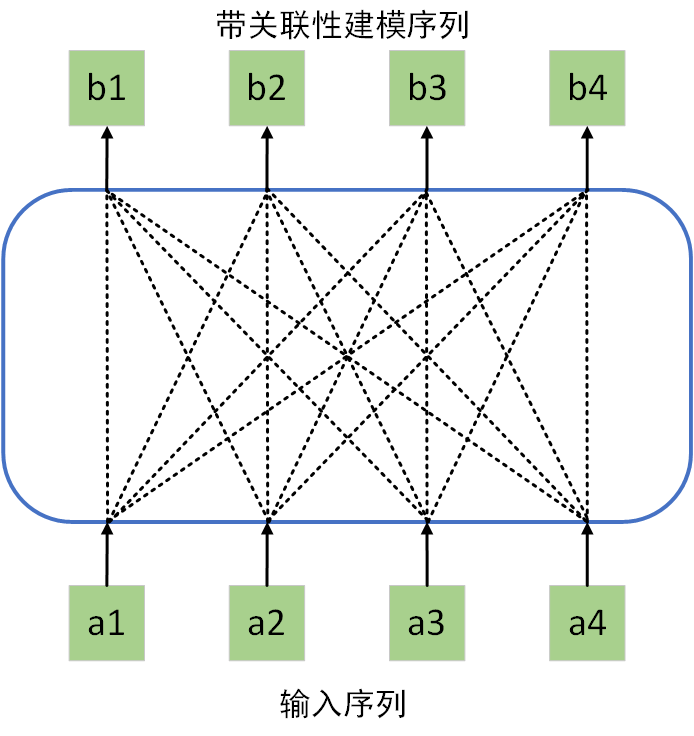
\includegraphics[width=0.6\textwidth]{Fig/myfig/chapter2/selfatt.png}  %scale = 0.3
	% 添加标签one_DFUAV以及图标题“XXX”,引用某图时使用\ref{xxx},其中xxx就是标签,图编号是自动生成的。
	\caption{\label{sys_need}自注意力机制} 
\end{figure}

\subsection{跨模态注意力}
跨模态注意力机制由Xu,Kelvin等人\cite{xu2015show}提出,是指利用注意力机制对来自不同模态的信息进行整合。它是深度学习中用于多模态数据融合的一种技术,数据可以来自不同的模态,如图像、文本或音频,跨模态注意力机制允许模型关注每个模态中与特定任务最相关的部分。
例如,在视觉问题回答(VQA)的背景下,该模型不但可以关注图像中的特定区域,同时也考虑问题文本以生成答案。该机制通过计算不同模态之间的注意分数来工作。
给定一个模态的输入,该模型计算出一组注意力权重,表明其他模态的每个元素的相关性。然后,注意力权重被用来计算其他模式元素的加权和,提供一个跨模式的表示,然后用于具体的下游任务。
\begin{figure}[htbp]
	% 图片居中(列居中对齐)
	\centering	
	% 包含当前路径下的Fig文件夹的图片文件
	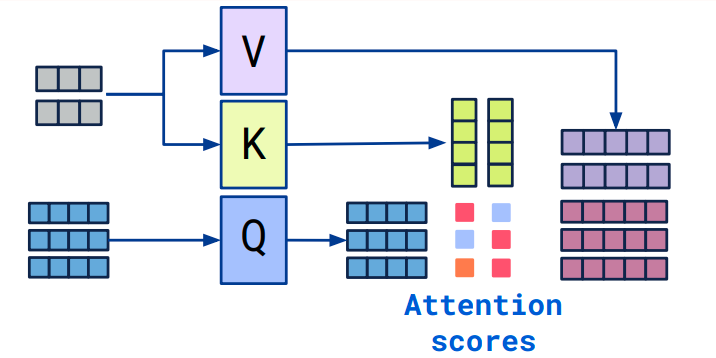
\includegraphics[width=1\textwidth]{Fig/myfig/chapter2/cross-attention.png}  %scale = 0.3
	% 添加标签one_DFUAV以及图标题“XXX”,引用某图时使用\ref{xxx},其中xxx就是标签,图编号是自动生成的。
	\caption{\label{sys_need}跨模态注意力机制} 
\end{figure}

\section{贝叶斯不确定性估计理论}
\subsection{贝叶斯定理}
贝叶斯定理是概率论中的一个基本公式,描述了在给定一些证据(观测值)的情况下,如何更新对一个事件发生的概率的估计。条件概率(又称后验概率)就是事件A在另外一个事件B已经发生条件下的发生概率。条件概率表示为P(A|B),读作“在B条件下A的概率”。
其计算方式可以描述为,假设在同一个样本空间Ω中的事件或者子集A与B,如果随机从Ω中选出的一个元素属于B,那么这个随机选择的元素还属于A的概率就定义为在B的前提下A的条件概率\eqref{bayes}:
\begin{equation}
	\label{bayes}
	P(A \mid B)=\frac{P(A \cap B)}{P(B)}
\end{equation}

$P(A)$和$P(B)$是事件A和B发生的先验概率,${P(A \cap B)}$是它们的联合概率。

\subsection{贝叶斯网络概述}
贝叶斯网络(Bayesian network),又称信念网络(Belief Network),或者有向无环模型,同时也是一种概率图模型,于1985年由Judea Pearl\cite{pearl1985bayesian}首先提出。它是一种模拟人类推理过程中因果关系的不确定性处理模型,其网络拓朴结构是一个有向无环图(DAG)。
图中的节点表示随机变量$\{X_1,X_2,...,X_n\}$,他们可以是可观察到的变量,隐变量,或者未知参数等。具有因果关系(或非条件独立)的变量或者命题则用箭头来连接。若两个节点间以一个单箭头连接,
表示两个节点之间是据因推果,则产生相应的一个条件概率值。

故而,把某个系统中涉及到的随机变量,根据是否条件独立绘制在一个有向图中,就形成了贝叶斯网络。该网络主要用来描述随机变量之间的条件依赖,对于任意的随机变量,其联合概率可以由各自的局部条件概率分布相乘而得出:
$$
P\left(x_1, \ldots, x_k\right)=P\left(x_k \mid x_1, \ldots, x_{k-1}\right) \ldots P\left(x_2 \mid x_1\right) P\left(x_1\right)
$$


% 它将贝叶斯框架引入神经网络,使其能够进行概率预测和估计不确定性。BNN能够对神经网络中的权重分布进行建模,这使得它们不仅能够生成点估计,而且能够生成输出的概率分布。
% 换句话说,BNN提供了一个鉴于观察数据和模型权重的先验概率分布的模型权重后验概率分布。
% \begin{figure}[htbp]
% 	% 图片居中(列居中对齐)
% 	\centering	
% 	% 包含当前路径下的Fig文件夹的图片文件
% 	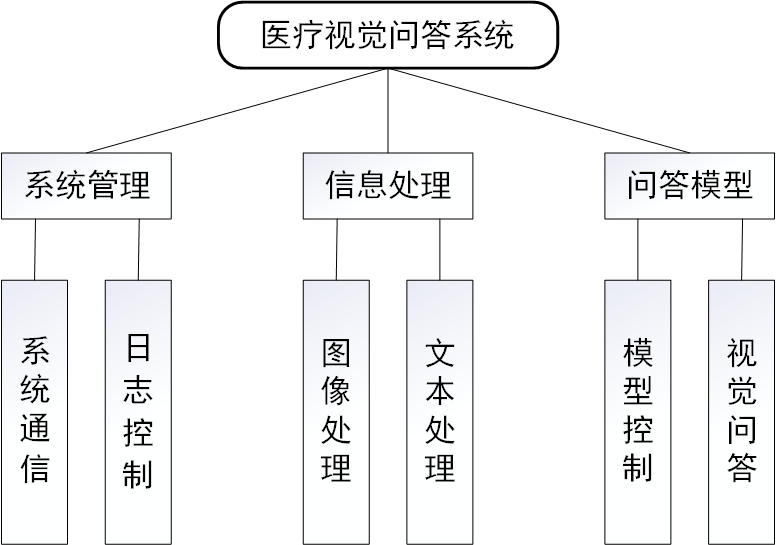
\includegraphics[width=0.8\textwidth]{Fig/myfig/chapter5/sys_need.png}  %scale = 0.3
% 	% 添加标签one_DFUAV以及图标题“XXX”,引用某图时使用\ref{xxx},其中xxx就是标签,图编号是自动生成的。
% 	\caption{\label{sys_need}需求分析} 
% \end{figure}

% 贝叶斯框架使BNN能够解决传统神经网络中的过拟合和缺乏鲁棒性的问题。通过对权重分布进行建模,BNNs可以做出对单个数据点不太敏感的预测,并在新数据上有更好的泛化性能。
% 此外,BNNs可以估计预测中的不确定性,这在医疗诊断、金融和自动驾驶等许多应用中非常有用。

\subsection{变分推断和蒙特卡洛方法}
变分推断(Variational Inference)和蒙特卡洛方法(Monte Carlo Methods)都是概率图模型中常用的推断方法。
变分推断是一种近似推断方法\cite{jordan1999introduction},通过在一族指定的分布族中寻找一个最接近真实后验分布的分布,从而近似后验分布。
具体来说,变分推断将后验分布近似为一个分布族 $q(\theta)$ 中与真实后验分布 $p(\theta|D)$ 最为接近的分布 $q^*(\theta)$,即最小化 $q(\theta)$ 与 $p(\theta|D)$ 之间的 KL 散度:
$$
\mathrm{KL}(q(\theta) \| p(\theta \mid D))=\int q(\theta) \log \frac{q(\theta)}{p(\theta \mid D)} \mathrm{d} \theta
$$
变分推断的目标就是寻找一个最优的 $q(\theta)$,使得 KL 散度最小。变分推断方法的优点是可以得到一个解析形式的近似后验分布,计算速度较快。但是由于对分布族的限制,其对真实后验分布的逼近能力有限。

蒙特卡洛方法\cite{metropolis1953equation}是一种基于采样的方法,通过从后验分布中采样得到样本,从而近似后验分布。常用的蒙特卡洛方法有马尔科夫链蒙特卡洛(MCMC)和重要性采样(Importance Sampling)等。
蒙特卡洛方法的优点是能够直接从后验分布中采样,对分布形态的限制较少,能够得到更加精确的后验分布近似。但是,蒙特卡洛方法在计算量上通常较大,需要进行大量的采样。

% \subsection{模态自适应原理}